\section{Introduction}

\subsection{Standard form}

\begin{frame}{Standard form}

    maximize $$\sum_{j=1}^{n}c_jx_j$$
    subject to 
        \begin{align*}
            \sum_{j=1}^{n}a_{ij}x_j\le b_i & \text{ for }i=1,2,\cdots,m\\
            x_j\ge 0 & \text{ for } j=1,2,\cdots, n
        \end{align*}

\end{frame}

\begin{frame}{Matrix form}

    maximize $$c^Tx$$
    subject to 
        \begin{align*}
            Ax\le b\\
            x\ge 0
        \end{align*}
    
\end{frame}

\begin{frame}{Converting linear programs into standard form}

    \begin{itemize}
        \item The objective function might be a minimization rather than a maximization.
        \item There might be variables without nonnegativity constraints.
        \item There might be equality constraints, which have an equal sign rather than a
        less-than-or-equal-to sign.
        \item There might be inequality constraints, but instead of having a 
        less-than-or-equal-to sign, they have a greater-than-or-equal-to sign.
    \end{itemize}
    
\end{frame}

\subsection{Terminology}

\begin{frame}{Terminology}

    \begin{itemize}
        \item \textbf{feasible solution} and \textbf{infeasible solution}
        \item $\bar{x}$ is an \textbf{optimal solution}, 
        we call $c^T\bar{x}$ the \textbf{optimal objective value}
        \item If a linear program has no feasible solutions, we say that the linear 
        program is \textbf{infeasible}; otherwise it is \textbf{feasible}.
        \item If a linear program has some feasible solutions but does not have a finite 
        optimal objective value, we say that the linear program is \textbf{unbounded}.
    \end{itemize}

\end{frame}

\subsection{Formulating problems as linear programs}

\begin{frame}{Shortest paths}

    \begin{figure}
        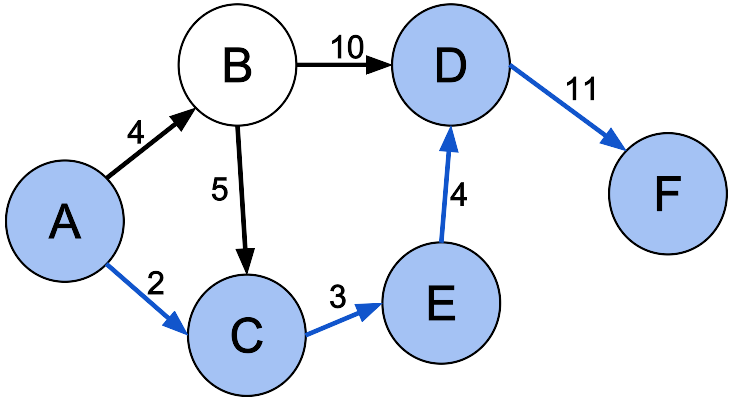
\includegraphics[width=0.5\textwidth]{assets/shortest_path.png}
        \caption{Shortest path problem}
    \end{figure}

    maximize $$d_t$$
    subject to 
    \begin{align*}
        d_v &\le d_u + w(u,v) \text{ for each edge }(u,v)\in E\\
        d_s &= 0
    \end{align*}

\end{frame}

\begin{frame}{Maximum flow}

    \begin{figure}
        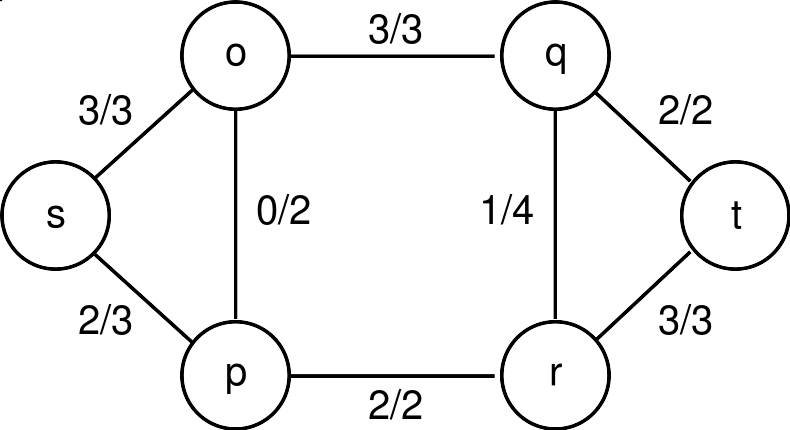
\includegraphics[width=0.3\textwidth]{assets/maximum_flow.png}
        \caption{Maximum flow problem}
    \end{figure}

    maximize $$\sum_{v\in V}f_{sv}-\sum_{v\in V}f_{vs}$$
    subject to 
    \begin{align*}
        f_{uv} &\le c(u,v) &\text{for each }u,v\in V\\
        \sum_{v\in V} f_{vu}&= \sum_{v\in V} f_{uv} &\text{for each } u\in V-\{s,t\}\\
        f_{uv}&\ge 0 &\text{for each }u,v\in V
    \end{align*}

\end{frame}
